\subsection*{Ход Работы}


\textbf{Темновая ВАХ}.
Измерим темновую ВАХ фотодиода, данные приведены в таблице 1, см. рис. \ref{fig:1}.


\begin{figure}[h]
    \centering
    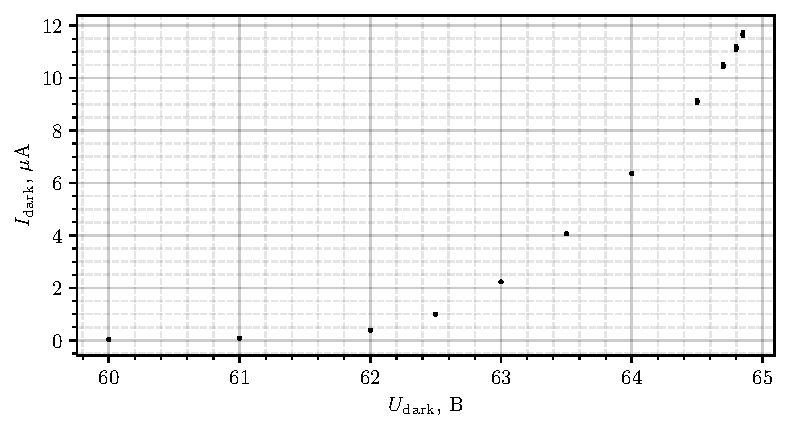
\includegraphics[width=0.75\textwidth]{figures/plot1.pdf}
    \caption{Темновая ВАХ фотодиода}
    \label{fig:1}
\end{figure}

 

\textbf{Настройка светодиода}.
Настроим интенсивность светодиода так, чтобы
\begin{equation*}
    \sub{I}{light}(20 \text{ В}) \approx \sub{I}{dark} (20 \text{ В}).
\end{equation*}
Для этого сначала было подано напряжение в 20 В на фотодетектор в обратном смещении, затем плавно увеличивалось неапряжение на светодиоде. 
Значение 20 В выбрано потому что оно соответствует полному формированию ОПЗ (области пространственного заряда). Коэффициент умножения $M(20 \text{ В}) = 1$. 


\textbf{Световая ВАХ}. Измерим световую ВАХ фотодиода, данные приведены в таблице 2, см. рис. \ref{fig:2}.

\begin{figure}[h]
    \centering
    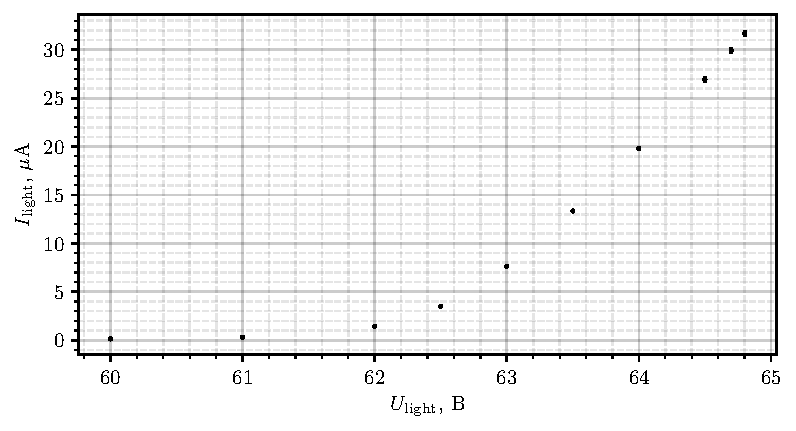
\includegraphics[width=0.75\textwidth]{figures/plot2.pdf}
    \caption{Световая ВАХ фотодиода}
    \label{fig:2}
\end{figure}

Напряжение $U$ измерялось достаточно точно, чтобы пренебречь погрешностью. Погрешность измерения тока $I$ была взята за 1\% в связи с нестаблильностью измеряемой величины.


\newpage

\textbf{Коэффициент лавинного умножения}. Значение фототока может быть найдено, как
\begin{equation*}
    \sub{I}{photo} (U_i) = \sub{I}{light} (U_i) - \sub{I}{dark}(U_i).
\end{equation*}
Тогда коэффициент лавинного умножения:
\begin{equation*}
    M(U_i) = \sub{I}{photo}(U_i) / \sub{I}{photo} (20 \text{ В}),
\end{equation*}
данные приведены в таблице 3. Построим зависимость $M(U_i)$, см. рис. \ref{fig:3}.

\begin{figure}[h]
    \centering
    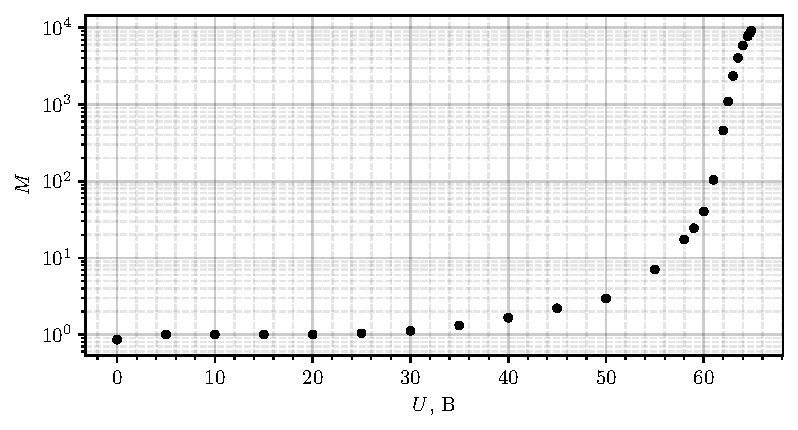
\includegraphics[width=0.75\textwidth]{figures/plot3.pdf}
    \caption{Зависость коэффициент лавинного умножения $M (U)$}
    \vspace{-5mm}
    \label{fig:3}
\end{figure}


Зависимость коэффициента лаинного умножения SiPM от перенапряжения в гейгероской области апроксимируется линейной функцией:
\begin{equation*}
    M(U) = \frac{C (U - \sub{U}{br})}{e}.
\end{equation*}
Построим лавинный участок $M(U)$ в линейном масштабе (см. рис. \ref{fig:4}) и аппроксимируем линейной функцией $M(U) = a U - b$. 

\begin{figure}[h]
    \centering
    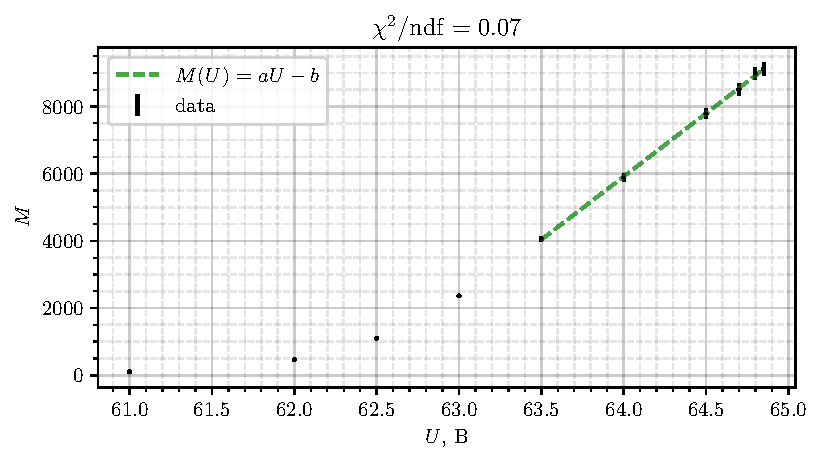
\includegraphics[width=0.75\textwidth]{figures/plot4.pdf}
    \vspace{-5mm}
    \caption{Лавинный участок зависимости $M(U)$}
    \label{fig:4}
\end{figure}

По  МНК находим коэффициенты аппроксимации:
\begin{equation*}
    a = (368 \pm 4) \times 10 \text{ В}^{-1},
    \hspace{10 mm} 
    b = (230 \pm 3) \times  10^3.
\end{equation*}
Из которых находим значения емкости ячейки и пробойное напряжение $\sub{U}{br}$:
\begin{equation*}
    C = e \cdot a = (0.59 \pm 0.02) \text{ фФ},
    \hspace{10 mm} 
    \sub{U}{br} = \frac{b}{a} = (62 \pm 2) \text{ В}.
\end{equation*}


